\documentclass[../main.tex]{subfiles}

\begin{document}
\chapter{Numerical Differentiation}

\vspace{1,5in}

\begin{center}\begin{Large}\textbf{CHAPTER OBJECTIVES}\end{Large}\end{center}
The primary objective of this chapter is to introduce you to numerical differentiation.
Specific objectives and topics covered are

\begin{itemize}
	\item Understanding the application of high-accuracy numerical differentiation
formulas for equispaced data.
	\item Knowing how to evaluate derivatives for unequally spaced data.
	\item Understanding how Richardson extrapolation is applied for numerical
differentiation.
	\item Recognizing the sensitivity of numerical differentiation to data error.
	\item Knowing how to evaluate derivatives in MATLAB with the diff and gradient
functions.
	\item Knowing how to generate contour plots and vector fields with MATLAB.
\end{itemize}
\vspace{0.3in}
\begin{Large}\textbf{YOU'VE GOT A PROBLEM}\end{Large}\\
Recall that the velocity of a free-falling bungee jumper as a function of time can be
computed as
\begin{equation}
	\tag{21.1}
	v(t) = \sqrt{\dfrac{gm}{c_{d}}} tanh \left( \sqrt{\dfrac{gc_{d}}{m} t} \right)
\end{equation}\\
At the beginning of Chap. 19, we used calculus to integrate this equation to determine the
vertical distance $z$ the jumper has fallen after a time $t$.
\begin{equation}
	\tag{21.2}
	z(t) = \dfrac{m}{c_{d}} ln \left[ cosh \left( \sqrt{\dfrac{gc_{d}}{m}} t \right) \right]
\end{equation}

Now suppose that you were given the reverse problem. That is, you were asked to determine velocity based on the jumper's position as a function of time. Because it is the inverse of integration, differentiation could be used to make the determination:
\begin{equation}
	\tag{21.3}
	v(t) = \dfrac{dz(t)}{dt}
\end{equation}\\
Substituting Eq. (21.2) into Eq. (21.3) and differentiating would bring us back to Eq. (21.1).

Beyond velocity, you might also be asked to compute the jumper's acceleration. To
do this, we could either take the first derivative of velocity, or the second derivative of
displacement:
\begin{equation}
	\tag{21.4}
	a(t) = \dfrac{dv(t)}{dt} = \dfrac{d^{2}z(t)}{dt^{2}}
\end{equation}\\
In either case, the result would be
\begin{equation}
	\tag{21.5}
	a(t) = g sech^{2} \left( \sqrt{\dfrac{gc_{d}}{m}}t \right)
\end{equation}

Although a closed-form solution can be developed for this case, there are other functions that may be difficult or impossible to differentiate analytically. Further, suppose that
there was some way to measure the jumper's position at various times during the fall.
These distances along with their associated times could be assembled as a table of discrete
values. In this situation, it would be useful to differentiate the discrete data to determine the
velocity and the acceleration. In both these instances, numerical differentiation methods
are available to obtain solutions. This chapter will introduce you to some of these methods.

\vspace{0,6in}
\section{INTRODUCTION AND BACKGROUND}
\vspace{0,1in}
\hrule
\vspace{0,1in}
\subsection{What Is Differentiation?}
$Calculus$ is the mathematics of change. Because engineers and scientists must continuously
deal with systems and processes that change, calculus is an essential tool of our profession.
Standing at the heart of calculus is the mathematical concept of differentiation.

According to the dictionary definition, to $differentiate$ means “to mark off by differences; distinguish; . . . to perceive the difference in or between.” Mathematically, the $derivative$, which serves as the fundamental vehicle for differentiation, represents the rate of change
of a dependent variable with respect to an independent variable. As depicted in Fig. 21.1, the
mathematical definition of the derivative begins with a difference approximation:
\begin{equation}
	\tag{21.6}
	\dfrac{\Delta y}{\Delta x} = \dfrac{f(x_{i} + \Delta x)-f(x_{i})}{\Delta x}
\end{equation}\\
where $y$ and $f=(x)$ are alternative representatives for the dependent variable and $x$ is the
independent variable. If x is allowed to approach zero, as occurs in moving from Fig. 21.1a
to c, the difference becomes a derivative:
\begin{equation}
	\tag{21.7}
	\dfrac{dy}{dx} = \lim \limits_{\Delta x \longrightarrow 0} \dfrac{f(x_{i} + \Delta x) - f(x_{i})}{\Delta x}
\end{equation}



\begin{figure}[hbt!]
	\centering
	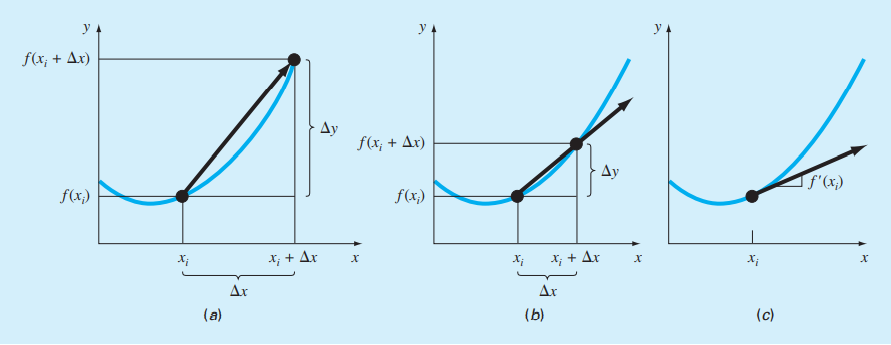
\includegraphics[width=0.65\textwidth]{pic.21.1}
	\caption{\textsf{The graphical definition of a derivative: as $\Delta x$ approaches zero in going from (a) to (c), the difference approximation
becomes a derivative. }} \hrule
	\label{pic.21.1}
\end{figure}
\pagebreak
where $dy/dx$ [which can also be designated as $y'$ or $f'(x_{i})]$\footnote{ The form $dy/dx$ was devised by Leibnitz, whereas $y$ is attributed to Lagrange. Note that Newton used the 
so-called dot notation: $y'$. Today, the dot notation is usually used for time derivatives.} is the first derivative of $y$ with
respect to $x$ evaluated at $x_{i}$. As seen in the visual depiction of Fig. 21.1c, the derivative is
the slope of the tangent to the curve at $x_{i}$.

The second derivative represents the derivative of the first derivative,
\begin{equation}
	\tag{21.8}
	\dfrac{d^{2} y}{dx^{2}} = \dfrac{d}{dx} \left( \dfrac{dy}{dx} \right)
\end{equation}\\
Thus, the second derivative tells us how fast the slope is changing. It is commonly referred
to as the $curvature$, because a high value for the second derivative means high curvature.

Finally, partial derivatives are used for functions that depend on more than one variable.
Partial derivatives can be thought of as taking the derivative of the function at a point with
all but one variable held constant. For example, given a function $f$ that depends on both $x$
and $y$, the partial derivative of f with respect to $x$ at an arbitrary point $(x, y)$ is defined as
\begin{equation}
	\tag{21.9}
	\dfrac{\partial f}{\partial x} = \lim \limits_{\Delta x \longrightarrow 0} \dfrac{f(x+ \Delta x, y) - f(x,y)}{\Delta x}
\end{equation}\\
Similarly, the partial derivative of $f$ with respect to $y$ is defined as
\begin{equation}
	\tag{21.10}
	\dfrac{\partial f}{\partial y} = \lim \limits_{\Delta \longrightarrow 0} \dfrac{f(x,y + \Delta y) - f(x,y)}{\Delta y}
\end{equation}

To get an intuitive grasp of partial derivatives, recognize that a function that depends on
two variables is a surface rather than a curve. Suppose you are mountain climbing and have
access to a function f that yields elevation as a function of longitude (the east-west oriented $x$ axis) and latitude (the north-south oriented $y$ axis). If you stop at a particular point $(x_{0}, y_{0})$,
the slope to the east would be $\partial f(x_{0},y_{0})/ \partial x$, and the slope to the north would be $\partial f(x_{0}, y_{0})/ \partial y$.

\subsection{Differentiation in Engineering and Science}
The differentiation of a function has so many engineering and scientific applications that
you were required to take differential calculus in your first year at college. Many specific examples of such applications could be given in all fields of engineering and science. Differentiation is commonplace in engineering and science because so much of our work involves
characterizing the changes of variables in both time and space. In fact, many of the laws and
other generalizations that figure so prominently in our work are based on the predictable
ways in which change manifests itself in the physical world. A prime example is Newton's
second law, which is not couched in terms of the position of an object but rather in its change
with respect to time.

Aside from such temporal examples, numerous laws involving the spatial behavior of
variables are expressed in terms of derivatives. Among the most common of these are the
$constitutive \, laws$ that define how potentials or gradients influence physical processes. For
example, $Fourier's \, law \, of \, heat \, conduction$ quantifies the observation that heat flows from
regions of high to low temperature. For the one-dimensional case, this can be expressed
mathematically as
\begin{equation}
	\tag{21.11}
	q = -k \dfrac{dT}{dx}
\end{equation}\\
where $q (x)$ = heat flux (W/m2
), $k$ = coefficient of thermal conductivity [W/(m · K)], T =
temperature (K), and $x$ = distance (m). Thus, the derivative, or $gradient$, provides a measure
of the intensity of the spatial temperature change, which drives the transfer of heat (Fig. 21.2).
\pagebreak
\begin{figure}[hbt!]
	\centering
	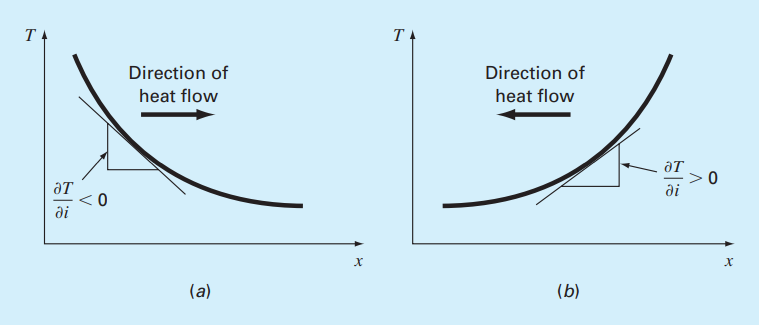
\includegraphics[width=0.75\textwidth]{pic.21.2}
	\caption{\textsf{FIGURE 21.2
Graphical depiction of a temperature gradient. Because heat moves “downhill” from high to low
temperature, the flow in (a) is from left to right. However, due to the orientation of Cartesian
coordinates, the slope is negative for this case. Thus, a negative gradient leads to a positive
flow. This is the origin of the minus sign in Fourier's law of heat conduction. The reverse case is
depicted in (b), where the positive gradient leads to a negative heat flow from right to left.}} \hrule
	\label{pic.21.2}
\end{figure}\\
\begin{table}[hbt!]
\caption{\textsf{The one-dimensional forms of some constitutive laws commonly used in
engineering and science.}} \hrule
\begin{tabular}{p{0.8in} c p{1.2in} cc p{0.9in}}
	
	\textbf{Law} & \textbf{Equation} & \textbf{Physical Area} & \textbf{Gradient} & \textbf{Flux} & \textbf{Proportionality}\\ \hrule
	
	Fourier's law & $q= -k \dfrac{dT}{dx}$ & Heat conduction &  Temperature & Heat flux & Thermal
Conductivity

\vspace{0,1in}\\

	Fick's law & $J=-D\dfrac{dc}{dx}$ & Mass diffusion & Concentration & Mass flux & Diffusivity\\
	
\vspace{0,1in}\\
	
	Darcy's law & $q=-k \dfrac{dh}{dx}$ & Flow through porous media & Head & Flow flux &  Hydraulic Conductivity\\
	
\vspace{0,1in}\\

	Ohm's law & $J=\sigma \dfrac{dV}{dx}$ & Current flow & Voltage & Current flux & Electrical
Conductivity\\

\vspace{0,1in}\\

	Newton's viscosity law & $\tau = \mu \dfrac{du}{dx}$ & Fluids & Velocity & Shear Stress & Dynamic Viscosity\\
	
\vspace{0,1in}\\	
	
	Hooke's law & $\sigma = E \dfrac{\Delta L}{L}$ & Elasticity & Deformation & Stress & Young's Modulus\\ \hrule
\end{tabular}
\end{table}

Similar laws provide workable models in many other areas of engineering and science,
including the modeling of fluid dynamics, mass transfer, chemical reaction kinetics, electricity, and solid mechanics (Table 21.1). The ability to accurately estimate derivatives is an
important facet of our capability to work effectively in these areas.

Beyond direct engineering and scientific applications, numerical differentiation is also
important in a variety of general mathematical contexts including other areas of numerical
methods. For example, recall that in Chap. 6 the secant method was based on a finitedifference approximation of the derivative. In addition, probably the most important application of numerical differentiation involves the solution of differential equations. We have
already seen an example in the form of Euler's method in Chap. 1. In Chap. 24, we will investigate how numerical differentiation provides the basis for solving boundary-value
problems of ordinary differential equations.

These are just a few of the applications of differentiation that you might face regularly
in the pursuit of your profession. When the functions to be analyzed are simple, you will normally choose to evaluate them analytically. However, it is often difficult or impossible when
the function is complicated. In addition, the underlying function is often unknown and defined only by measurement at discrete points. For both these cases, you must have the ability
to obtain approximate values for derivatives, using numerical techniques as described next.

\vspace{0,6in}
\section{HIGH-ACCURACY DIFFERENTIATION FORMULAS}
\vspace{0,1in}
\hrule
\vspace{0,1in}
We have already introduced the notion of numerical differentiation in Chap. 4. Recall that
we employed Taylor series expansions to derive finite-difference approximations of derivatives. In Chap. 4, we developed forward, backward, and centered difference approximations
of first and higher derivatives. Remember that, at best, these estimates had errors that were $O(h^{2})$ -that is, their errors were proportional to the square of the step size. This level of
accuracy is due to the number of terms of the Taylor series that were retained during the derivation of these formulas. We will now illustrate how high-accuracy finite-difference formulas can be generated by including additional terms from the Taylor series expansion.

For example, the forward Taylor series expansion can be written as [recall Eq. (4.13)]
\begin{equation}
	\tag{21.12}
	f(x_{i+1}) = f(x_{i}) + f'(x_{i})h + \dfrac{f''(x_{i})}{2!}h^{2} + \cdots
\end{equation}\\
which can be solved for
\begin{equation}
	\tag{21.13}
	f'(x_{i})= \dfrac{f(x_{i+1})-f(x_{i})}{h} - \dfrac{f''(x_{i})}{2!}h + O(h^{2})
\end{equation}\\
In Chap. 4, we truncated this result by excluding the second- and higher-derivative terms
and were thus left with a forward-difference formula:
\begin{equation}
	\tag{21.14}
	f'(x_{i}) = \dfrac{f(x_{i+1})-f(x_{i})}{h} + O(h)
\end{equation}

In contrast to this approach, we now retain the second-derivative term by substituting
the following forward-difference approximation of the second derivative [recall Eq. (4.27)]:
\begin{equation}
	\tag{21.15}
	f''(x_{i})=\dfrac{f(x_{i+2})-2f(x{i+1}) + f(x_{i}}{h^{2}} + O(h)
\end{equation}\\
into Eq. (21.13) to yield
\begin{equation}
	\tag{21.16}
	f'(x_{i})=\dfrac{f(x_{i+1})-f(x_{i})}{h}-\dfrac{ f(x_{i+2}) -2f(x_{i+1})  + f(x_{i})  }{ 2h^{2} } h + O(h^{2})
\end{equation}\\
or, by collecting terms:
\begin{equation}
	\tag{21.17}
	f'(x_{i}) = \dfrac{ -f(x_{i+2}) +4f(x_{i+1}) -3f(x_{i}) }{ 2h } + O(h^{2})
\end{equation}

Notice that inclusion of the second-derivative term has improved the accuracy to $O(h^{2})$.
Similar improved versions can be developed for the backward and centered formulas as
well as for the approximations of higher-order derivatives. The formulas are summarized in
Fig. 21.3 through Fig. 21.5 along with the lower-order versions from Chap. 4. The following example illustrates the utility of these formulas for estimating derivatives. 

\vspace{0,6in}
\section{High-Accuracy Differentiation Formulas}
\vspace{0,1in}
\hrule
\vspace{0,1in}
\textbf{Problem Statement.} Recall that in Example 4.4 we estimated the derivative of

	$$f(x) = -0.1x^{4} - 0.15x^{3} - 0.5x^{2} 0.25x +1.2$$\\
at $x$ = 0.5 using finite-differences and a step size of $h$ = 0.25. The results are summarized
in the following table. Note that the errors are based on the true value of
$f' (0.5) = −0.9125$.

\begin{table}[hbt!]
\centering
\begin{tabular}{lccc}
\hline
	\vspace{0,1in} & \textbf{Backward $O(h)$} & \textbf{Centered $O(h^{2})$} & \textbf{Forward $O(h)$}\\ \hline
	
	\textbf{Estimate} & −0.714 & −0.934 & −1.155\\
	
	$\varepsilon_{t}$ & 21.7\% & −2.4\% & −26.5\%\\ \hline
\end{tabular}
\end{table}
Repeat this computation, but employ the high-accuracy formulas from Fig. 21.3 through
Fig. 21.5.

\begin{figure}[hbt!]
	\centering
	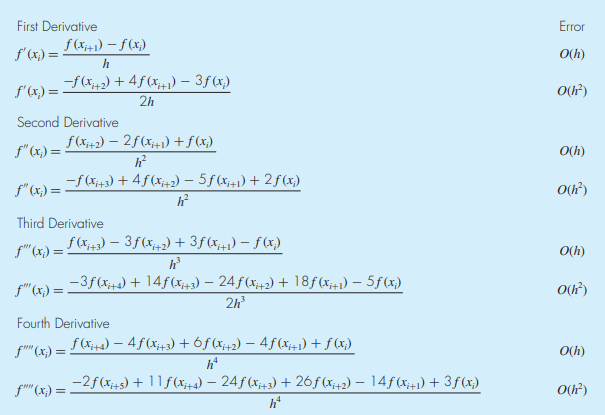
\includegraphics[width=0.75\textwidth]{pic.21.3}
	\caption{\textsf{Forward finite-difference formulas: two versions are presented for each derivative. The latter version
incorporates more terms of the Taylor series expansion and is, consequently, more accurate.}} \hrule
	\label{pic.21.3}
\end{figure}
\vspace{0.2in}
\textbf{Solution.} The data needed for this example are

\begin{tabular}{ll}
	
	$x_{i-2} = 0$ & $f(x_{i-2}) = 1.2$\\
	
	$x_{i-1} = 0.25$ & $f(x_{i-2}) = 1.1035156$\\
	
	$x_{i} = 0.5$ & $f(x_{i}) = 0.925$\\
	
	$x_{i+1} = 0.75$ & $f(x_{i+1}) = 0.6363281$\\
	
	$x_{i+2} = 1$ & $f(x_{i+2}) = 0.2$
\end{tabular}\\
\vspace{0.2in}\\
The forward difference of accuracy O(h2) is computed as (Fig. 21.3)

	$$f'(0.5) = \dfrac{-0.2 + 4(0.6363281) -3(0.925) }{ 2(0.25)} = - 0.859375 \; \; \; \; \; \; \varepsilon_{t}=5.82\%$$\\
The backward difference of accuracy $O(h^{2})$ is computed as (Fig. 21.4)

	$$f'(0.5) = \dfrac{3(0.925) - 4(1.1035156) + 1.2}{2(0.25)} = -0.878125 \; \; \; \; \; \; \varepsilon_{t} = 3.77\%$$\\
The centered difference of accuracy O(h4) is computed as (Fig. 21.5)

	$$f'(0.5) = \dfrac{-0.2 + 8((0.6363281) -  8(1.1035156) + 1.2}{12(0.25)} -0.9125 \; \; \; \; \; \varepsilon_{t} = 5.82\%$$
	
\begin{figure}[hbt!]
	\centering
	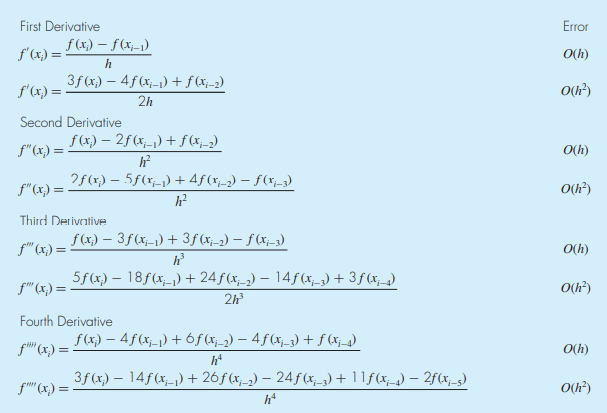
\includegraphics[width=0.75\textwidth]{pic.21.4}
	\caption{\textsf{Backward finite-difference formulas: two versions are presented for each derivative. The latter
version incorporates more terms of the Taylor series expansion and is, consequently, more accurate.}} \hrule
	\label{pic.21.4}
\end{figure}

\vspace{0.2in}

As expected, the errors for the forward and backward differences are considerably
more accurate than the results from Example 4.4. However, surprisingly, the centered difference yields the exact derivative at $x$ = 0.5. This is because the formula based on the
Taylor series is equivalent to passing a fourth-order polynomial through the data points.

\section{RICHARDSON EXTRAPOLATION}
To this point, we have seen that there are two ways to improve derivative estimates when
employing finite differences: (1) decrease the step size or (2) use a higher-order formula
that employs more points. A third approach, based on Richardson extrapolation, uses two
derivative estimates to compute a third, more accurate, approximation.

Recall from Sec. 20.2.1 that Richardson extrapolation provided a means to obtain an
improved integral estimate by the formula [Eq. (20.4)]
\begin{equation}
	\tag{21.18}
	I = I(h_{2}) + \dfrac{1}{(h_{1}/h_{2})^{2} -1} [I(h_{2}) - I(h_{1})]
\end{equation}\\
where $I(h_{1})$ and $I(h_{2})$ are integral estimates using two step sizes: $h_{1}$ and $h_{2}$. Because of
its convenience when expressed as a computer algorithm, this formula is usually written
for the case where $h_{2} = h_{1}/2$, as in
\begin{equation}
	\tag{21.19}
	I=\dfrac{4}{3}I(h_{2}) - \dfrac{1}{3}I(h_{1})
\end{equation}

\begin{figure}[hbt!]
	\centering
	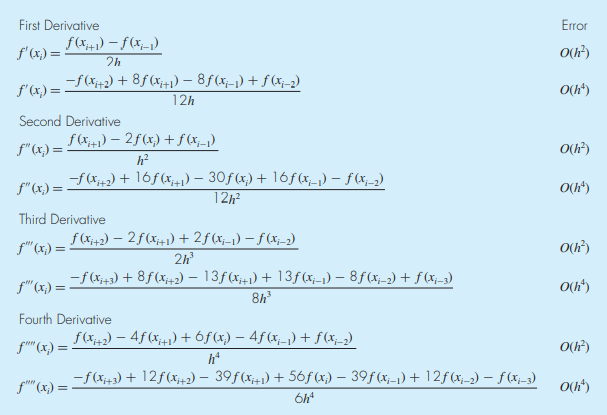
\includegraphics[width=0.75\textwidth]{pic.21.5}
	\caption{\textsf{Centered finite-difference formulas: two versions are presented for each derivative. The latter
version incorporates more terms of the Taylor series expansion and is, consequently, more
accurate.
}} \hrule
	\label{pic.21.5}
\end{figure}
In a similar fashion, Eq. (21.19) can be written for derivatives as
\begin{equation}
	\tag{21.20}
	D= \dfrac{4}{3}D(h_{2}) - \dfrac{1}{3}D(h_{1})
\end{equation}\\
For centered difference approximations with O(h2), the application of this formula will
yield a new derivative estimate of $O(h_{4})$.

\vspace{0,6in}
\section{Richardson Extrapolation}
\vspace{0,1in}
\hrule
\vspace{0,1in}
\textbf{Problem Statement.} Using the same function as in Example 21.1, estimate the first derivative at $x$ = 0.5 employing step sizes of $h_{1}$ = 0.5 and $h_{2}$ = 0.25. Then use Eq. (21.20)
to compute an improved estimate with Richardson extrapolation. Recall that the true value
is −0.9125.\\
\vspace{0.2in}\\
\textbf{Solution.} The first-derivative estimates can be computed with centered differences as

	$$D(0.5) = \dfrac{0.2 - 1.2}{1} = - 1.0 \; \; \; \; \; \varepsilon_{t} = -9.6\%$$\\
and

	$$D(0.25) = \dfrac{0.6363281 - 1.103516}{0.5} = -0.934375 \; \; \; \; \; \varepsilon_{t} = -2.4\%$$\\
The improved estimate can be determined by applying Eq. (21.20) to give

	$$D = \dfrac{4}{3}(-0.934375) -\dfrac{1}{3}(-1) = -0.9125$$\\
which for the present case is exact.
\vspace{0.2in}

The previous example yielded an exact result because the function being analyzed was
a fourth-order polynomial. The exact outcome was due to the fact that Richardson extrapolation is actually equivalent to fitting a higher-order polynomial through the data and then
evaluating the derivatives by centered divided differences. Thus, the present case matched
the derivative of the fourth-order polynomial precisely. For most other functions, of course,
this would not occur, and our derivative estimate would be improved but not exact. Consequently, as was the case for the application of Richardson extrapolation, the approach can
be applied iteratively using a Romberg algorithm until the result falls below an acceptable
error criterion. 

\vspace{0,6in}
\section{DERIVATIVES OF UNEQUALLY SPACED DATA}
\vspace{0,1in}
\hrule
\vspace{0,1in}
The approaches discussed to this point are primarily designed to determine the derivative of
a given function. For the finite-difference approximations of Sec. 21.2, the data had to be
evenly spaced. For the Richardson extrapolation technique of Sec. 21.3, the data also had to
be evenly spaced and generated for successively halved intervals. Such control of data spacing is usually available only in cases where we can use a function to generate a table of values.

In contrast, empirically derived information—that is, data from experiments or field
studies—are often collected at unequal intervals. Such information cannot be analyzed
with the techniques discussed to this point.

One way to handle nonequispaced data is to fit a Lagrange interpolating polynomial
[recall Eq. (17.21)] to a set of adjacent points that bracket the location value at which you
want to evaluate the derivative. Remember that this polynomial does not require that the
points be equispaced. The polynomial can then be differentiated analytically to yield a formula that can be used to estimate the derivative.

For example, you can fit a second-order Lagrange polynomial to three adjacent points
($x_{0}$, $y_{0}$),($x_{1}$, $y_{1}$), and ($x_{2}$, $y_{2}$). Differentiating the polynomial yields:
\begin{equation}
	\tag{21.21}
	f'(x) = f(x_{0})\dfrac{2x - x_{1} - x_{2}}{(x_{0} - x_{1}) (x_{0} - x_{2})} + f(x_{1})\dfrac{2x - x_{0} - x_{2}}{(x_{1}-x_{0})(x_{1} - x_{2})} + f(x_{2})\dfrac{2x-x_{0} - x_{1}}{(x_{2} - x_{0}) (x_{2} - x_{1})}
\end{equation}\\
where x is the value at which you want to estimate the derivative. Although this equation is
certainly more complicated than the first-derivative approximation from Fig. 21.3 through
Fig. 21.5, it has some important advantages. First, it can provide estimates anywhere
within the range prescribed by the three points. Second, the points themselves do not have
to be equally spaced. Third, the derivative estimate is of the same accuracy as the centered
difference [Eq. (4.25)]. In fact, for equispaced points, Eq. (21.21) evaluated at $x = x_{1}$ reduces to Eq. (4.25).

\vspace{0,6in}
\section{Differentiating Unequally Spaced Data}
\vspace{0,1in}
\hrule
\vspace{0,1in}
\textbf{Problem Statement.} As in Fig. 21.6, a temperature gradient can be measured down into the
soil. The heat flux at the soil-air interface can be computed with Fourier's law (Table 21.1):

	$$q(z=0) = -k \dfrac{dT}{dz} \bigg| _{z=0}$$\\
where $q(z)$ = heat flux ($W/m^{2}$), $k$ = coefficient of thermal conductivity for soil [= 0.5 W/
(m · K)], $T$ = temperature (K), and $z$ = distance measured down from the surface into the
soil (m). Note that a positive value for flux means that heat is transferred from the air to the
soil. Use numerical differentiation to evaluate the gradient at the soil-air interface and employ this estimate to determine the heat flux into the ground.


\vspace{0.4in}
\textbf{Solution.} Equation (21.21) can be used to calculate the derivative at the air-soil interface as

\begin{table}[hbt!]
\begin{tabular}{l p{5.1in}}
\vspace{0,1in} & $f'(0) = 13.5\dfrac{2(0)-0.0125 - 0.0375}{(0 − 0.0125)(0 − 0.0375)} + 12\dfrac{2(0) − 0 − 0.0375}{(0.0125 − 0)(0.0125 − 0.0375)} +10\dfrac{2(0) − 0 − 0.0125}{(0.0375 − 0)(0.0375 − 0.0125)} =  −1440 + 1440 − 133.333 = −133.333 K/m$\\
\end{tabular}
\end{table}
which can be used to compute

	$$q(z=0) = -0.5 \dfrac{W}{mK} \left( -133.333 \dfrac{K}{m} \right) = 66.667 \dfrac{W}{m^{2}}$$

\begin{figure}[hbt!]
	\hrule
	\caption{\textsf{Temperature versus depth into the soil.}} 
	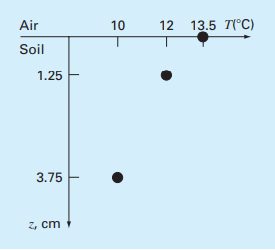
\includegraphics[width=0.45\textwidth]{pic.21.6}
	\label{pic.21.6}
\end{figure}

\vspace{0,6in}
\section{DERIVATIVES AND INTEGRALS FOR DATA WITH ERRORS}
\vspace{0,1in}
\hrule
\vspace{0,1in}
Aside from unequal spacing, another problem related to differentiating empirical data is
that these data usually include measurement error. A shortcoming of numerical differentiation is that it tends to amplify errors in the data.

\begin{figure}[hbt!]
	\centering
	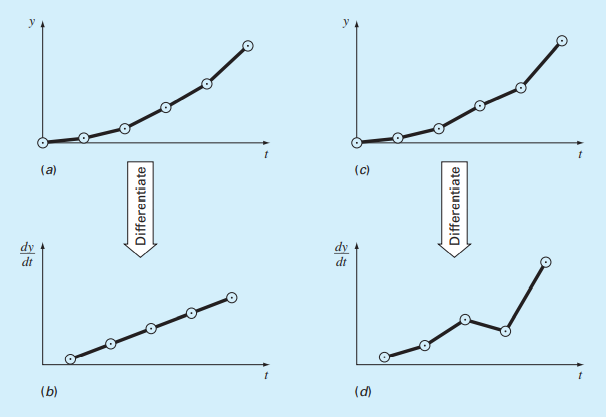
\includegraphics[width=0.75\textwidth]{pic.21.7}
	\caption{\textsf{Illustration of how small data errors are amplified by numerical differentiation: (a) data with no
error, (b) the resulting numerical differentiation of curve (a), (c) data modified slightly, and (d) the
resulting differentiation of curve (c) manifesting increased variability. In contrast, the reverse
operation of integration [moving from (d) to (c) by taking the area under (d)] tends to attenuate 
or smooth data errors.}} \hrule
	\label{pic.21.7}
\end{figure}

Fig. 21.7a shows smooth, error-free data that when numerically differentiated yield
a smooth result (Fig. 21.7b). In contrast, Fig. 21.7c uses the same data, but with alternating points raised and lowered slightly. This minor modification is barely apparent from
Fig. 21.7c. However, the resulting effect in Fig. 21.7d is significant.

The error amplification occurs because differentiation is subtractive. Hence, random
positive and negative errors tend to add. In contrast, the fact that integration is a summing
process makes it very forgiving with regard to uncertain data. In essence, as points are
summed to form an integral, random positive and negative errors cancel out.

As might be expected, the primary approach for determining derivatives for imprecise
data is to use least-squares regression to fit a smooth, differentiable function to the data. In
the absence of any other information, a lower-order polynomial regression might be a good
first choice. Obviously, if the true functional relationship between the dependent and independent variable is known, this relationship should form the basis for the least-squares fit.

\vspace{0,6in}
\section{PARTIAL DERIVATIVES}
\vspace{0,1in}
\hrule
\vspace{0,1in}

Partial derivatives along a single dimension are computed in the same fashion as ordinary
derivatives. For example, suppose that we want to determine to partial derivatives for a
two-dimensional function $f (x, y)$. For equally spaced data, the partial first derivatives can be approximated with centered differences:
\begin{equation}
	\tag{21.22}
	\dfrac{\partial f}{\partial x} = \dfrac{f(x + \Delta x, y) - f(x- \Delta x, y)}{2\Delta x}
\end{equation}
\begin{equation}
	\tag{21.23}
	\dfrac{\partial f}{\partial y} = \dfrac{f(x,y+\Delta y) - f(x,y - \Delta y)}{2 \Delta y}
\end{equation}\\
All the other formulas and approaches discussed to this point can be applied to evaluate
partial derivatives in a similar fashion.

For higher-order derivatives, we might want to differentiate a function with respect to
two or more different variables. The result is called a $mixed\, partial\, derivative$. For example, we might want to take the partial derivative of f (x, y) with respect to both independent
variables
\begin{equation}
	\tag{21.24}
	\dfrac{\partial^{2} f}{\partial x \partial y} = \dfrac{\partial}{\partial x} \left( \dfrac{\partial f}{\partial y} \right)
\end{equation}\\
To develop a finite-difference approximation, we can first form a difference in $x$ of the partial derivatives in $y$:
\begin{equation}
	\tag{21.25}
	\dfrac{\partial^{2} f}{\partial x \partial y} = \dfrac{\dfrac{\partial f}{\partial y} (x + \Delta x,y) - \dfrac{\partial f}{\partial y} (x - \Delta x, y)}{2\Delta x}
\end{equation}\\
Then, we can use finite differences to evaluate each of the partials in $y$:
\begin{equation}
	\tag{21.26}
	\dfrac{\partial^{2} f}{\partial x \partial y} = \dfrac{ \dfrac{f(x+\Delta x, y + \Delta y) - f(x+\Delta x, y - \Delta y)} {2 \Delta y} - \dfrac {f(x - \Delta x, y + \Delta y) - f(x - \Delta x,y - \Delta y)}{2 \Delta y}}{2\Delta y}
\end{equation}\\
Collecting terms yields the final result
\begin{equation}
	\tag{21.27}
	\dfrac{\partial^{2} f}{\partial x \partial y} = \dfrac{ f(x + \Delta x, y+ \Delta y) - f(x+ \Delta x, y-\Delta ) - f(x-\Delta x,y+ \Delta y) + f(x - \Delta x, y- \Delta y)}{4 \Delta x \Delta y}
\end{equation}

\vspace{0,6in}
\section{NUMERICAL DIFFERENTIATION WITH MATLAB}
\vspace{0,1in}
\hrule
\vspace{0,1in}

MATLAB software has the ability to determine the derivatives of data based on two builtin functions: diff and gradient. 

\subsection{MATLAB Function: diff}
When it is passed a one-dimensional vector of length $n$, the diff function returns a vector
of length $n − 1$ containing the differences between adjacent elements. As described in the
following example, these can then be employed to determine finite-difference approximations of first derivatives.

\vspace{0,6in}
\section{Using diff for Differentiation}
\vspace{0,1in}
\hrule
\vspace{0,1in}

\textbf{Problem Statement.} Explore how the MATLAB diff function can be employed to differentiate the function

	$$f(x) = 0.2 + 25x - 200x^{2} + 675x^{3} - 900x^{4} + 400x^{5}$$\\
from $x$ = 0 to 0.8. Compare your results with the exact solution:

	$$f'(x) = 25 - 400x^{2} + 2025x^{2} - 3600x^{3} + 2000x^{4}$$
	
\textbf{Solution.} We can first express $f(x)$ as an anonymous function:

\begin{verbatim}
   >> f=@(x) 0.2+25*x-200*x.^2+675*x.^3-900*x.^4+400*x.^5;
\end{verbatim}
We can then generate a series of equally spaced values of the independent and dependent
variables:
\begin{verbatim}
   >> x=0:0.1:0.8;
   >> y=f(x);
\end{verbatim}
The diff function can be used to determine the differences between adjacent elements of
each vector. For example,
\begin{verbatim}
   
   >> diff(x)
   ans =
     Columns 1 through 5
       0.1000 0.1000 0.1000 0.1000 0.1000
     Columns 6 through 8
       0.1000 0.1000 0.1000
\end{verbatim}
As expected, the result represents the differences between each pair of elements of x. To
compute divided-difference approximations of the derivative, we merely perform a vector
division of the y differences by the x differences by entering
\begin{verbatim}
   >> d=diff(y)./diff(x)
   d =
     Columns 1 through 5
       10.8900 -0.0100 3.1900 8.4900 8.6900
     Columns 6 through 8
       1.3900 -11.0100 -21.3100
\end{verbatim}
Note that because we are using equally spaced values, after generating the x values, we
could have simply performed the above computation concisely as
\begin{verbatim}
   >> d=diff(f(x))/0.1;
\end{verbatim}

The vector $d$ now contains derivative estimates corresponding to the midpoint between adjacent elements. Therefore, in order to develop a plot of our results, we must first
generate a vector holding the $x$ values for the midpoint of each interval:

\begin{verbatim}
   >> n=length(x);
   >> xm=(x(1:n-1)+x(2:n))./2;
\end{verbatim}
\pagebreak
\begin{figure}[hbt!]
	\centering
	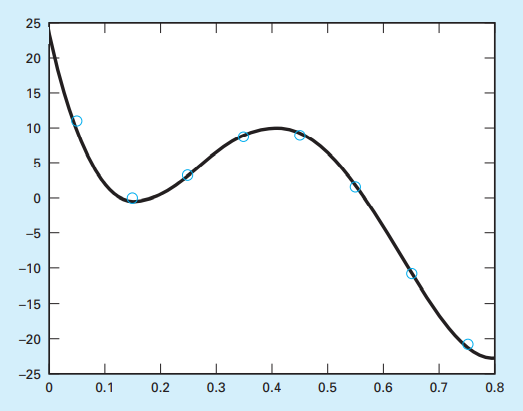
\includegraphics[width=0.55\textwidth]{pic.21.8}
	\caption{\textsf{Comparison of the exact derivative (line) with numerical estimates (circles) computed with
MATLAB's diff function.}} \vspace{0.1in} \hrule
	\label{pic.21.8}
\end{figure}
As a final step, we can compute values for the analytical derivative at a finer level of resolution to include on the plot for comparison

\begin{verbatim}
   >> xa=0:.01:.8;
   >> ya=25-400*xa+3*675*xa.^2-4*900*xa.^3+5*400*xa.^4;
\end{verbatim}
A plot of the numerical and analytical estimates can be generated with
\begin{verbatim}
   >> plot(xm,d,'o',xa,ya)
\end{verbatim}
As displayed in Fig. 21.8, the results compare favorably for this case.
\vspace{0.4in}

Note that aside from evaluating derivatives, the diff function comes in handy as a
programming tool for testing certain characteristics of vectors. For example, the following
statement displays an error message and terminates an M-file if it determines that a vector
$x$ has unequal spacing:
\begin{verbatim}
   if any(diff(diff(x))~=0), error('unequal spacing'), end
\end{verbatim}

Another common use is to detect whether a vector is in ascending or descending order.
For example, the following code rejects a vector that is not in ascending order (that is, monotonically increasing):
\begin{verbatim}
   if any(diff(x)<=0), error('not in ascending order'), end
\end{verbatim}

\subsection{MATLAB Function: gradient }
The gradient function also returns differences. However, it does so in a manner that is
more compatible with evaluating derivatives at the values themselves rather than in the
intervals between values. A simple representation of its syntax is 
\begin{verbatim}
   fx = gradient(f)
\end{verbatim}
where $f = a$ one-dimensional vector of length $n$, and $fx$ is a vector of length $n$ containing
differences based on $f$. Just as with the diff function, the first value returned is the difference between the first and second value. However, for the intermediate values, a centered difference based on the adjacent values is return

\begin{equation}
	\tag{21.28}
	diff_{i} = \dfrac{f_{i+1} - f_{i-1}}{2}
\end{equation}\\
The last value is then computed as the difference between the final two values. Hence, the
results are akin to using centered differences for all the intermediate values, with forward
and backward differences at the ends. 

Note that the spacing between points is assumed to be one. If the vector represents
equally spaced data, the following version divides all the results by the interval and hence
returns the actual values of the derivatives,
\begin{verbatim}
   fx = gradient(f, h)
\end{verbatim}
where $h$ = the spacing between points.

\vspace{0,6in}

\section{Using gradient for Differentiation}

\vspace{0,1in}
\hrule
\vspace{0,1in}

\textbf{Problem Statement.} Use the gradient function to differentiate the same function that
we analyzed in Example 21.4 with the diff function.

\textbf{Solution.} In the same fashion as Example 21.4, we can generate a series of equally
spaced values of the independent and dependent variables:

\begin{verbatim}
   >> f=@(x) 0.2+25*x-200*x.^2+675*x.^3-900*x.^4+400*x.^5;
   >> x=0:0.1:0.8;
   >> y=f(x);
\end{verbatim}
We can then use the gradient function to determine the derivatives as
\begin{verbatim}
   >> dy=gradient(y,0.1)
   dy =
     Columns 1 through 5
      10.8900 5.4400 1.5900 5.8400 8.5900
     Columns 6 through 9
       5.0400   -4.8100   -16.1600   -21.3100
\end{verbatim}
As in Example 21.4, we can generate values for the analytical derivative and display both
the numerical and analytical estimates on a plot:
\begin{verbatim}
   >> xa=0:.01:.8;
   >> ya=25-400*xa+3*675*xa.^2-4*900*xa.^3+5*400*xa.^4;
   >> plot(x,dy,'o', xa,ya)
\end{verbatim}
\pagebreak
\begin{figure}[hbt!]
	\centering
	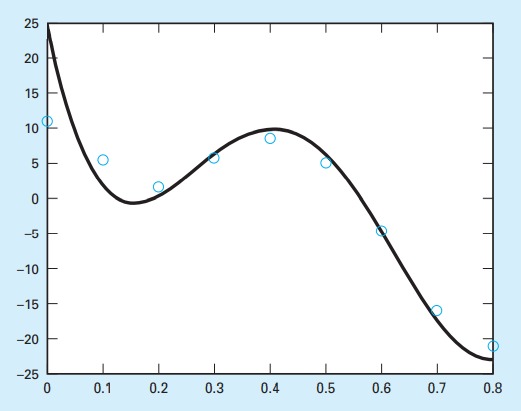
\includegraphics[width=0.60\textwidth]{pic.21.9}
	\caption{\textsf{Comparison of the exact derivative (line) with numerical estimates (circles) computed with
MATLAB's gradient function.}} \vspace{0.1in} \hrule 
	\label{pic.21.9}
\end{figure}
\vspace{0.2in}

As displayed in Fig. 21.9, the results are not as accurate as those obtained with the
diff function in Example 21.4. This is due to the fact that gradient employs intervals
that are two times (0.2) as wide as for those used for diff (0.1).

\vspace{0.4in}
Beyond one-dimensional vectors, the gradient function is particularly well suited
for determining the partial derivatives of matrices. For example, for a two-dimensional matrix, $f$, the function can be invoked as
\begin{verbatim}
   [fx,fy] = gradient(f, h)
\end{verbatim}
where $fx$ corresponds to the differences in the $x$ (column) direction, and $fy$ corresponds
to the differences in the $y$ (row) direction, and $h$ = the spacing between points. If $h$ is
omitted, the spacing between points in both dimensions is assumed to be one. In the next
section, we will illustrate how gradient can be used to visualize vector fields.

\vspace{0,6in}
\section{CASE STUDY VISUALIZING FIELDS}
\vspace{0,1in}
\hrule
\vspace{0,1in}
\textbf{Background.} Beyond the determination of derivatives in one dimension, the gradient
function is also quite useful for determining partial derivatives in two or more dimensions.
In particular, it can be used in conjunction with other MATLAB functions to produce visualizations of vector fields.

To understand how this is done, we can return to our discussion of partial derivatives
at the end of Section 21.1.1. Recall that we used mountain elevation as an example of a
two-dimensional function. We can represent such a function mathematically as

	$$z=f(x,y)$$\\
where $z$ = elevation, $x$ = distance measured along the east-west axis, and $y$ = distance
measured along the north-south axis.

For this example, the partial derivatives provide the slopes in the directions of the
axes. However, if you were mountain climbing, you would probably be much more interested in determining the direction of the maximum slope. If we think of the two partial derivatives as component vectors, the answer is provided very neatly by 

	$$\triangledown f = \dfrac{\partial f}{\partial x} \textbf{i} + \dfrac{\partial f}{\partial y} \textbf{j}$$\\
where $\triangledown f$ is referred to as the $gradient$ of $f$. This vector, which represents the steepest
slope, has a magnitude

	$$\sqrt{\left(\dfrac{\partial f}{\partial x} \right)^{2} + \left( \dfrac{\partial f}{\partial y} \right)^{2}}$$\\
and a direction

	$$\theta = \tan^{1} \left( \dfrac{\partial f/ \partial y}{\partial f / \partial x} \right)$$\\
where $\theta$ = the angle measured counterclockwise from the $x$ axis. 

Now suppose that we generate a grid of points in the $x-y$ plane and used the foregoing
equations to draw the gradient vector at each point. The result would be a field of arrows
indicating the steepest route to the peak from any point. Conversely, if we plotted the negative of the gradient, it would indicate how a ball would travel as it rolled downhill from
any point.

Such graphical representations are so useful that MATLAB has a special function,
called quiver, to create such plots. A simple representation of its syntax is
\begin{verbatim}
   quiver(x,y,u,v)
\end{verbatim}
where $x$ and $y$ are matrices containing the position coordinates and $u$ and $v$ are matrices
containing the partial derivatives. The following example demonstrates the use of quiver
to visualize a field.

Employ the gradient function to determine to partial derivatives for the following
two-dimensional function:

	$$f(x,y) = y-x-2x^{2} - 2xy - y^{2}$$\\
from $x$ = −2 to 2 and $y$ = 1 to 3. Then use quiver to superimpose a vector field on a contour plot of the function.\\
\textbf{Solution.} We can first express $f(x, y)$ as an anonymous function
\begin{verbatim}
   >> f=@(x,y) y-x-2*x.^2-2.*x.*y-y.^2;
\end{verbatim}
A series of equally spaced values of the independent and dependent variables can be generated as
\begin{verbatim}
   >> [x,y]=meshgrid(-2:.25:0, 1:.25:3);
   >> z=f(x,y);
\end{verbatim}
The gradient function can be employed to determine the partial derivatives:
\begin{verbatim}
   >> [fx,fy]=gradient(z,0.25);
\end{verbatim}
We can then develop a contour plot of the results:
\begin{verbatim}
   >> cs=contour(x,y,z);clabel(cs);hold on
\end{verbatim}
As a final step, the resultant of the partial derivatives can be superimposed as vectors on the
contour plot:
\begin{verbatim}
   >> quiver(x,y,-fx,-fy);hold off
\end{verbatim}

\begin{figure}[hbt!]
	\caption{\textsf{MATLAB generated contour plot of a two-dimensional function with the resultant of the partial
derivatives displayed as arrows.}} \hrule \vspace{0.2in}
\centering
	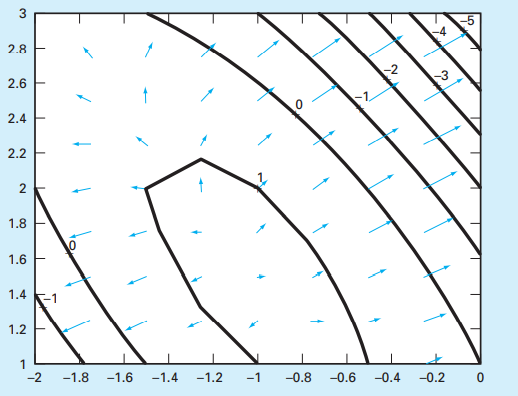
\includegraphics[width=0.65\textwidth]{pic.21.10}
	\label{pic.21.10}
\end{figure}
Note that we have displayed the negative of the resultants, in order that they point 
“downhill.”

The result is shown in Fig. 21.10. The function's peak occurs at $x$ = −1 and $y$ = 1.5
and then drops away in all directions. As indicated by the lengthening arrows, the gradient
drops off more steeply to the northeast and the southwest.

\subsection*{PROBLEMS} \hrule

\begin{multicols}{2}
\textbf{21.1} Compute forward and backward difference approximations of $O(h)$ and $O(h^{2})$, and central difference approximations of $O(h^{2})$ and $O(h^{4})$ for the first derivative of
$y = \cos x$ at $x = \pi/4$ using a value of $h = \pi/12$. Estimate
the true percent relative error εt for each approximation. 

\textbf{21.2} Use centered difference approximations to estimate the
first and second derivatives of $y = e^{x}$ at $x = 2$ for $h = 0.1$.
Employ both $O(h^{2})$ and $O(h^{4})$ formulas for your estimates.

\textbf{21.3} Use a Taylor series expansion to derive a centered
finite-difference approximation to the third derivative that is
second-order accurate. To do this, you will have to use four
different expansions for the points $x_{i-2}$,$x_{i-1}$, $x_{i+1}$, and $x_{i+2}$. In each case, the expansion will be around the point $x_{i}$.  The
interval $\Delta x$ will be used in each case of $i$ − 1 and $i$ + 1, and $2\Delta x$ will be used in each case of $i$ − 2 and $i$ + 2. The four
equations must then be combined in a way to eliminate the
first and second derivatives. Carry enough terms along in
each expansion to evaluate the first term that will be truncated to determine the order of the approximation. 

\textbf{21.4} Use Richardson extrapolation to estimate the first derivative of $y = \cos x$ at $x = \pi/4$ using step sizes of $h_{1} = \pi/3$ and $h_{2} = \pi/6$. Employ centered differences of $O(h^{2})$ for the
initial estimates.

\textbf{21.5} Repeat Prob. 21.4, but for the first derivative of ln $x$ at
$x$ = 5 using $h_{1}$ = 2 and $h_{2}$ = 1.

\textbf{21.6} Employ Eq. (21.21) to determine the first derivative 
of $y = 2x4 − 6x3 − 12x − 8$ at $x = 0$ based on values at $x_{0} = - 0.5$, $x_{1} = 1$, and $x_{2} = 2$. Compare this result with
the true value and with an estimate obtained using a centered
difference approximation based on $h$ = 1.

\textbf{21.7} Prove that for equispaced data points, Eq. (21.21)
reduces to Eq. (4.25) at $x = x_{1}$.

\textbf{21.8} Develop an M-file to apply a Romberg algorithm to
estimate the derivative of a given function.

\textbf{21.9} Develop an M-file to obtain first-derivative estimates
for unequally spaced data. Test it with the following data: \\
\begin{tabular}{lccccc}
	\hline
{\textbf{$x$}} & {0.6} & {1.5} & {1.6} & {2.5} & {3.5}\\
{\textbf{$f(x)$}} & {0.9036} & {0.3734} & {0.3261} & {0.08422} & {0.01596}\\ \hline
\end{tabular} \vspace{0.1in} \\
where $f (x) = 5e^{−2x} x$ . Compare your results with the true
derivatives.

\textbf{21.10} Develop an M-file function that computes first and
second derivative estimates of order $O(h^{2})$ based on the formulas in Figs. 21.3 through 21.5. The function's first line
should be set up as
\begin{verbatim}
   function [dydx, d2ydx2] = diffeq(x,y)
\end{verbatim}
where $x$ and $y$ are input vectors of length $n$ containing the
values of the independent and dependent variables, respectively, and $dydx$ and $dy2dx2$ are output vectors of length $n$
containing the first- and second-derivative estimates at
each value of the independent variable. The function should
generate a plot of $dydx$ and $dy2dx2$ versus $x$. Have your 
M-file return an error message if \textbf{(a)} the input vectors are not
the same length, or \textbf{(b)} the values for the independent variable are not equally spaced. Test your program with the data
from Prob. 21.11.

\textbf{21.11} The following data were collected for the distance
traveled versus time for a rocket: \\ 
\begin{tabular}{lcccccc}
\hline
\textbf{$t,s$} \; & \; 0 \; & \; 25 \; & \; 50 \; & \; 75 \;
 & \; 100 & 125\\ 
\textbf{$y, km$} & 0 & 32 & 58 & 78 & 92 & 100\\ \hline
\end{tabular} \vspace{0.1in} \\
Use numerical differentiation to estimate the rocket's velocity and acceleration at each time. 

\textbf{21.12} A jet fighter's position on an aircraft carrier's runway
was timed during landing: \\
\begin{tabular}{lccccccc}
\hline
\textbf{$t, s$} & 0 & 0.52 & 1.04 & 1.75 & 2.37 & 3.25 & 3.83\\ 
\textbf{$x, m$} & 153 & 185 & 208 & 249 & 261 & 271 & 273\\  \hline
\end{tabular}\\
where x is the distance from the end of the carrier. Estimate
\textbf{(a)} velocity $(dx/dt)$ and \textbf{(b)} acceleration $(dv/dt)$ using numerical differentiation.

\textbf{21.13} Use the following data to find the velocity and acceleration at $t$ = 10 seconds:\\
\begin{tabular}{lccccccccc}
	\hline
	
	\tiny{\textbf{$Time, t, s$}} & \tiny{0} & \tiny{2} & \tiny{4} & \tiny{6} & \tiny{8} & \tiny{10} & \tiny{12} & \tiny{14} & \tiny{16}\\

	\tiny{\textbf{$Position, x, m$}} & \tiny{0} & \tiny{0.7} & \tiny{1.8} & \tiny{3.4} & \tiny{5.1} & \tiny{6.3} & \tiny{7.3} & \tiny{8.0} & \tiny{8.4}\\ \hline
\end{tabular}\\
Use second-order correct \textbf{(a)} centered finite-difference, 
\textbf{(b)} forward finite-difference, and \textbf{(c)} backward finitedifference methods.

\textbf{21.14} A plane is being tracked by radar, and data are taken
every second in polar coordinates $\theta$ and $r$.\\
\begin{tabular}{lcccccc}
\hline

	{\textbf{$ t $, s}} & {200} & {202} & {204} & {206} & {208} & {21C}\\
	
	{\textbf{$\theta$, (rad)}} & {0.75} & {0.72} & {0.70} & {0.68} & {0.67} & {0.66}\\
	
	{\textbf{$ r $, m}} & {5120} & {5370} & {5560} & {5800} & {6030} & {6240}\\
		
\hline
\end{tabular}
At 206 seconds, use the centered finite-difference (secondorder correct) to find the vector expressions for velocity v
and acceleration a. The velocity and acceleration given in
polar coordinates are

$\vec{v} = \dot{r} \vec{e}_{r} + r \dot{\theta} \vec{e}_{\theta} \; \; \; \; \textit{and} \; \; \; \; \vec{a} = (\ddot{r} - r \dot{\theta}^{2}) \vec{e}_{r} + (r \ddot{\theta} + 2\vec{r} \vec{\theta} \vec{e}_{\theta} $\\

\textbf{21.15} Use regression to estimate the acceleration at each
time for the following data with second-, third-, and fourthorder polynomials. Plot the results:\\
\begin{tabular}{lcccccccccc}
\hline

	{\textbf{t}} & {1} & {2} & {3.25} & {4.5} & {6} & {7} & {8} & {8.5} & {9.3} & {10}\\
	
	{\textbf{v}} & {10} & {12} & {11} & {14} & {17} & {16} & {12} & {14} & {14} & {10}\\

	\hline
\end{tabular}\

\textbf{21.16} The normal distribution is defined as

	$$f(x) = \dfrac{1}{\sqrt{2\pi}} e^{-x^{2} / 2}$$\
Use MATLAB to determine the inflection points of this
function. 

\textbf{21.17} The following data were generated from the normal
distribution:\\
\begin{tabular}{lccccc}
\hline

	\footnotesize{\textbf{x}} & \footnotesize{-2} & \footnotesize{-1.5} & \footnotesize{-1} & \footnotesize{-0.5} & \footnotesize{0}\\
	
	\footnotesize{\textbf{f(x)}} & \footnotesize{0.05399} & \footnotesize{0.12952} & \footnotesize{0.24197} & \footnotesize{0.35207} & \footnotesize{0.39894}\\
	
	\vspace{0,1in}\\
	
	\footnotesize{\textbf{x}} & \footnotesize{0.5} & \footnotesize{1} & \footnotesize{1.5} & \footnotesize{2} & \vspace{0,1in}\\
	
	\footnotesize{\textbf{f(x)}} & \footnotesize{0.35207} & \footnotesize{0.24197} & \footnotesize{0.12952} & \footnotesize{0.05399} & \vspace{0,1in}\\

\hline
\end{tabular}\
Use MATLAB to estimate the inflection points of these data.

\textbf{21.18} Use the \texttt{diff(y)}  command to develop a MATLAB
M-file function to compute finite-difference approximations
to the first and second derivative at each x value in the table
below. Use finite-difference approximations that are second order correct, $O (x^{2})$:\\
\begin{tabular}{lccccccccccc}
\hline

	\tiny{\textbf{x}} & \tiny{0} & \tiny{1} & \tiny{2} & \tiny{3} & \tiny{4} & \tiny{5} & \tiny{6} & \tiny{7} & \tiny{8} & \tiny{9} & \tiny{10}\\
	
	\tiny{\textbf{y}} & \tiny{1.4} & \tiny{2.1} & \tiny{3.3} & \tiny{4.8} & \tiny{6.8} & \tiny{6.6} & \tiny{8.6} & \tiny{7.5} & \tiny{8.9} & \tiny{10.9} & \tiny{10}\\

\hline
\end{tabular}

\textbf{21.19} The objective of this problem is to compare secondorder accurate forward, backward, and centered finitedifference approximations of the first derivative of a function
to the actual value of the derivative. This will be done for

	$$f(x) = e^{-2x} - x$$

\begin{enumerate}
	\item[\textbf{(a)}] Use calculus to determine the correct value of the derivative at $x = 2$
	
	\item[\textbf{(b)}] Develop an M-file function to evaluate the centered
finite-difference approximations, starting with $x=0.5$. Thus, for the first evaluation, the $x$ values for the centered difference approximation will be $x = 2 \pm 0.5$ or
$x = 1.5$ and $2.5$. Then, decrease in increments of $0.1$
down to a minimum value of $\Delta x = 0.01$.

	\item[\textbf{(c)}] Repeat part \textbf{(b)} for the second-order forward and backward differences. (Note that these can be done at the same
time that the centered difference is computed in the loop.)
 
	\item[\textbf{(d)}] Plot the results of \textbf{(b)} and \textbf{(c)} versus $x$. Include the exact
result on the plot for comparison. 
\end{enumerate}

\textbf{21.20} You have to measure the flow rate of water through a
small pipe. In order to do it, you place a bucket at the pipe's
outlet and measure the volume in the bucket as a function of
time as tabulated below. Estimate the flow rate at $t = 7$ s.\\
\begin{tabular}{lcccc}
\hline

	{\textbf{Time, s}} & {0} & {1} & {5} & {8}\\
	
	{\textbf{Volume, $cm^{3}$}} & {0} & {1} & {8} & {16.4}\\

\hline
\end{tabular}

\textbf{21.21} The velocity $v$ (m/s) of air flowing past a flat surface
is measured at several distances y (m) away from the surface. Use $Newton's viscosity law$ to determine the shear stress $\tau (N/m^{2})$ at the surface $(y=0)$,

$ \tau = \mu \dfrac{du}{dy} $\
Assume a value of dynamic viscosity $\mu = 1.8 x 10^{-5} N \cdot{} s/m^{2}$.\\
\begin{tabular}{lcccccc}
\hline

	{\textbf{$y$, m}} & {0} & {0.002} & {0.006} & {0.012} & {0.018} & {0.024}\\
	
	{\textbf{$u$, m/s}} & {0} & {0.287} & {0.899} & {1.915} & {3.048} & {4.299}\\
	
\hline
\end{tabular}

\textbf{21.22} $Fick's first diffusion law$ states that
\begin{equation}
\tag{P21.22}
\textrm{Mass ux} = -D\dfrac{dc}{dx}
\end{equation}\\
where mass flux = the quantity of mass that passes across a
unit area per unit time $(g/cm^{2}/s), D=a$ diffusion coefficient $(cm^{2}/s), c = \textrm \; {concentration} (g/cm^{3}), \; \textrm{and} \; x = \textrm{distance} \; (cm)$. An environmental engineer measures the following concentration of a pollutant in the pore waters of sediments underlying a lake ($x = 0$ at the sediment-water interface and
increases downward): \\
\begin{tabular}{lcccc}
\hline

	\textbf{$x$, cm} & \vspace{0,1in} & 0 & 1 & 3\\
	
	\textbf{$c, 10^{-6} g/cm^{3}$} & \vspace{0,1in} & 0.06 & 0.32 & 0.6\\

\hline
\end{tabular}\\
Use the best numerical differentiation technique available to
estimate the derivative at $x = 0$. Employ this estimate in
conjunction with Eq. (P21.22) to compute the mass flux of
pollutant out of the sediments and into the overlying waters $(D=1.52 x 10^{-6} cm^{2}/s)$. For a lake with $3.6 x 10^{6} m^{2}$ of
sediments, how much pollutant would be transported into
the lake over a year's time? 

\textbf{21.23} The following data were collected when a large oil
tanker was loading: \\
\begin{tabular}{lccccccc}
	\hline

	\scriptsize{\textbf{$t$, min}} & \scriptsize{0} & \scriptsize{10} & \scriptsize{20} & \scriptsize{30} & \scriptsize{45} & \scriptsize{60} & \scriptsize{75}\\
	
	\scriptsize{$V$, $10^{6}$ barrels} & \scriptsize{0.4} & \scriptsize{0.7} & \scriptsize{0.77} & \scriptsize{0.88} & \scriptsize{1.05} & \scriptsize{1.17} & \scriptsize{1.35}\\

	\hline
\end{tabular}\\
Calculate the flow rate $Q$ (i.e., $dV/dt$) for each time to the
order of $h^{2}$.

\textbf{21.24} Fourier's law is used routinely by architectural engineers to determine heat flow through walls. The following
temperatures are measured from the surface $(x = 0)$ into a
stone wall: \\
\begin{tabular}{lcccccccccccc}
	\hline

	$x$, m & \vspace{0,1in} & \vspace{0,1in} & \vspace{0,1in} & 0 & \vspace{0,1in} & \vspace{0,1in} & \vspace{0,1in} & 0.08 & \vspace{0,1in} & \vspace{0,1in} & \vspace{0,1in} & 0.16\\
	
	$T$, $^{\circ}C$ & \vspace{0,1in} & \vspace{0,1in} & \vspace{0,1in} & 19 & \vspace{0,1in} & \vspace{0,1in} & \vspace{0,1in} & 17 & \vspace{0,1in} & \vspace{0,1in} & \vspace{0,1in} & 15\\


	\hline
\end{tabular}\\
If the flux at $x = 0$ is $60 W/m^2$, compute $k$.

\textbf{21.25} The horizontal surface area $A_{s} (m^2)$ of a lake at a particular depth can be computed from volume by differentiation: 

$A_{s}(z) = \dfrac{dV}{dz} (z)$
\\
where V = volume ($m^3$) and $z$ = depth (m) as measured
from the surface down to the bottom. The average concentration of a substance that varies with depth, $\overline{c} (g/m^3)$, can be
computed by integration:

$\overline{c} = \dfrac{\int^{Z}_{0} c(z) A_{s}(z)dz}  {\int^{Z}_{0} A_{s}(z)dz   }$
\\
where $Z$ = the total depth (m). Determine the average concentration based on the following data:\\
\begin{tabular}{lccccc}
	\hline

	\footnotesize{\textbf{$z$, m}} & \footnotesize{0} & \footnotesize{4} & \footnotesize{8} & \footnotesize{12} & \footnotesize{16}\\
	
	\footnotesize{\textbf{$V, 10^{6} m^3$}} & \footnotesize\footnotesize{9.8175} & \footnotesize{5.1051} & \footnotesize{1.9635} & \footnotesize{0.3927} & \footnotesize{0.0000}\\
	
	\footnotesize{$c, g/m^3$} & \footnotesize{10.2} & \footnotesize{8.5} & \footnotesize{7.4} & \footnotesize{5.2} & \footnotesize{4.1}\\ 

	\hline
\end{tabular}

\textbf{21.26} Faraday's law characterizes the voltage drop across
an inductor as

$V_{L} = L\dfrac{di}{dt}$
\\
where $V_{L}$ = voltage drop (V), L = inductance (in henrys; 
1 H = 1 V · s/A), i = current (A), and t = time (s). Determine the voltage drop as a function of time from the following data for an inductance of 4 H.
\\
\begin{tabular}{lcccccc}
	\hline

	$t$ \; & 0 \; & 0.1 \; & 0.2 \; & 0.3 \; & 0.5 \; & 0.7\\
	
	$i$ \; & 0 \; & 0.16 \; & 0.32 \; & 0.56 \; & 0.84 \; & 2.0\\

	\hline
\end{tabular}
\\


\textbf{21.27} Based on Faraday's law (Prob. 21.26), use the following voltage data to estimate the inductance if a current of 2 A
is passed through the inductor over 400 milliseconds.\\
\begin{tabular}{lcccccccccc}
	\hline

	 \tiny{\textbf{$t$, ms}} &  \tiny{0} &  \tiny{10} &  \tiny{20} &  \tiny{40} &  \tiny{60} &  \tiny{80} &  \tiny{120} &  \tiny{180} &  \tiny{280} &  \tiny{400}\\
	 
	 \tiny{\textbf{$V$, volts}} & \tiny{0} & \tiny{18} & \tiny{29} & \tiny{44} & \tiny{49} & \tiny{46} & \tiny{35} & \tiny{26} & \tiny{15} & \tiny{7}\\	

	 \hline
\end{tabular}

\textbf{21.28} The rate of cooling of a body (Fig. P21.28) can be expressed as

$\dfrac{dT}{dt} = -k(T-T_{a})$
\\
where $T$ = temperature of the body ($^{\circ}C$), $T_{a}$ = temperature of
the surrounding medium ($^{\circ}C$), and $k = a$ proportionality constant (per minute). Thus, this equation (called $Newton's law of cooling$) specifies that the rate of cooling is proportional to


\end{multicols}
\begin{figure}[hbt!]
	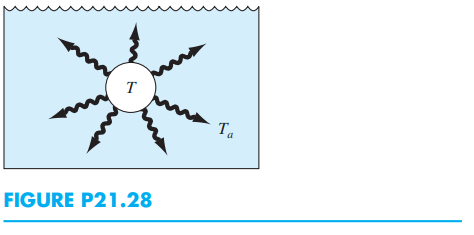
\includegraphics[width=0.50\textwidth]{pic.21.28}
	\label{pic.21.28}
\end{figure}
\begin{multicols}{2}
the difference in the temperatures of the body and of the surrounding medium. If a metal ball heated to $80 ^{\circ}C$ is dropped
into water that is held constant at $T_{a} = 20 ^{\circ}C$, the temperature
of the ball changes, as in\\
\begin{tabular}{lcccccc}
	\hline

	{\textbf{Time, min}} & {0} & {5} & {10} & {15} & {20} & {25}\\
	
	{\textbf{$T,^{\circ}$C}} & {80} & {44.5} & {30.0} & {24.1} & {21.7} & {20.7}\\
	
	\hline
\end{tabular}\\
\\
Utilize numerical differentiation to determine $dT/dt$ at each
value of time. Plot $dT/dt$ versus $T - T_{a}$ and employ linear
regression to evaluate $k$.

\textbf{21.29} The enthalpy of a real gas is a function of pressure as
described below. The data were taken for a real fluid. Estimate the enthalpy of the fluid at 400 K and 50 atm (evaluate
the integral from 0.1 atm to 50 atm).

$H = \int^{P}_{0} \left(V - T \left( \dfrac{\partial V}{\partial T} \right)_{P}\right)dP  $\\
\\
\\
\begin{tabular}{cccc}
	\hline
\vspace{0,1in}

	\vspace{0,1in} & \vspace{0,1in} & $V$, L & \vspace{0,1in}\\
	
	\hline
	
	\textbf{$P$, atm} & \textbf{$T$ = 350 K} & \textbf{$T$ = 400 K} & \textbf{$T$ = 450 K}\\
	
	\hline
	
	0.1 & 220 & 250 & 282.5\\
	5 & 4.1 & 4.7 & 5.23\\
	10 & 2.2 & 2.5 & 2.7\\
	20 & 1.35 & 1.49 & 1.55\\
	25 & 1.1 & 1.2 & 1.24\\
	30 & 0.90 & 0.99 & 1.03\\
	40 & 0.68 & 0.75 & 0.78\\
	45 & 0.61 & 0.675 & 0.7\\
	50 & 0.54 & 0.6 & 0.62\\
		
	
	\hline
\end{tabular}

\vspace{0,15 cm}

\textbf{21.30} For fluid flow over a surface, the heat flux to the surface can be computed with Fourier's law: y = distance normal to the surface (m). The following measurements are made for air flowing over a flat plate where y = distance normal to the surface:\\
\begin{tabular}{lcccc}
	\hline

	\textbf{$y$, cm} & 0 & 1 & 3 & 5\\
	
	\textbf{$T$}, K & 900 & 480 & 270 & 210\\
	
	\hline
\end{tabular}\\
If the plate's dimensions are 200 cm long and 50 cm wide,
and $k = 0.028 J/(s · m · K)$, \textbf{(a)} determine the flux at the surface, and \textbf{(b)} the heat transfer in watts. Note that 1 J = 1 W· s.

\textbf{21.31} The pressure gradient for laminar flow through a constant radius tube is given by

$\dfrac{dp}{dx} = - \dfrac{8\mu Q}{\pi r^4}$\\
where $p$ = pressure ($N/m^2$), $x$ = distance along the tube's
centerline (m), $μ$ = dynamic viscosity ($N · s/m^2$), $Q$ = flow
$(m^3/s)$ and r = radius (m).
\begin{enumerate}
	\item[\textbf{(a)}] Determine the pressure drop for a 10-cm length tube
for a viscous liquid ($μ = 0.005 N · s/m^2, density = ρ = 1 × 103 kg/m^3$) with a flow of $10 × 10−6 m^3/s$ and the following varying radii along its length: 
\end{enumerate}
\begin{tabular}{lccccccc}
\hline

	\textbf{$x$, cm} & 0 & 2 & 4 & 5 & 6 & 7 & 10\\
	\textbf{$r$, mm} & 2 & 1.35 & 134 & 1.6 & 1.58 & 1.42 & 2\\

\hline
\end{tabular}\\
\begin{enumerate}
	\item[\textbf{(b)}]Compare your result with the pressure drop that would
have occurred if the tube had a constant radius equal to
the average radius.

	\item[\textbf{(c)}] Determine the average Reynolds number for the tube to
verify that flow is truly laminar ($Re = \rho vD/\mu < 2100$
where $v$ = velocity).
\end{enumerate}


\textbf{21.32} The following data for the specific heat of benzene
were generated with an $n$th-order polynomial. Use numerical differentiation to determine $n$.\\
\begin{tabular}{lcccc}
	\hline

	\tiny{\textbf{$T$, K}} & \tiny{300} & \tiny{400} & \tiny{500} & \tiny{600}\\
	
	\tiny{\textbf{$C_{p}$, kJ/(kmol $\cdot$ K)}} &  \tiny{82.888} & \tiny{112.136} & \tiny{136.933} & \tiny{157.744}\\
	
	\vspace{0,1in}\\
	
	\tiny{\textbf{$T$, K}} & \tiny{700} & \tiny{800} & \tiny{900} & \tiny{1000}\\
	
	\tiny{\textbf{$C_{p}$, kJ/(kmol $\cdot$ K)}} & \tiny{175.036} & \tiny{189.273} & \tiny{200.923} & \tiny{210.450}\\

	\hline
\end{tabular}

\textbf{21.33} The specific heat at constant pressure $c_{p}$ [J/(kg · K)]
of an ideal gas is related to enthalpy by

  $ c_{p} = \dfrac{dh}{dT} $\\
where $h$ = enthalpy (kJ/kg), and $T$ = absolute temperature (K). The following enthalpies are provided for carbon dioxide ($CO_{2}$) at several temperatures. Use these values to
determine the specific heat in J/(kg · K) for each of the tabulated temperatures. Note that the atomic weights of carbon
and oxygen are 12.011 and 15.9994 g/mol, respectively\\
\begin{tabular}{lcccc}
	\hline

	\textbf{$T$, K} & 750 & 800 & 900 & 1000\\
	
	\textbf{$h$, kJ/kmol} & 29,629 & 32,179 & 37,405 & 42,769\\

	\hline
\end{tabular}


\textbf{21.34} An $n$th-order rate law is often used to model chemical
reactions that solely depend on the concentration of a single
reactant:

$ \dfrac{dc}{dt} = -kc^{n} $\\
where $c$ = concentration (mole), $t$ = time (min), $n$ =
reaction order (dimensionless), and $k$ = reaction rate 
($min^{−1}$ $mole^{1−n}$). The differential method can be used to
evaluate the parameters k and n. This involves applying a
logarithmic transform to the rate law to yield,

$ \log \left(-\dfrac{dc}{dt} \right) = \log k + n \log c $\\
Therefore, if the $n$th-order rate law holds, a plot of the
log($−dc/dt$) versus log $c$ should yield a straight line with a
slope of $n$ and an intercept of log $k$. Use the differential
method and linear regression to determine $k$ and $n$ for the
following data for the conversion of ammonium cyanate to
urea:\\
\begin{tabular}{lccccc}
	\hline

	\textbf{$t$, min} & 0 & 5 & 15 & 30 & 45\\

	\textbf{$c$, mole} & 0.750 & 0.594 & 0.420 & 0.291 & 0.223\\
	
	\hline
\end{tabular}


\textbf{21.35} The sediment oxygen demand [SOD in units of
$g/(m^2 · d)$] is an important parameter in determining the
dissolved oxygen content of a natural water. It is measured
by placing a sediment core in a cylindrical container 
(Fig. P21.35). After carefully introducing a layer of distilled,
oxygenated water above the sediments, the container is covered to prevent gas transfer. A stirrer is used to mix the water
gently, and an oxygen probe tracks how the water's oxygen
concentration decreases over time. The SOD can then be
computed as

$ \textnormal{SOD} = -H\dfrac{do}{dt} $\\
where $H$ = the depth of water (m), $o$ = oxygen concentration
($g/m^3$), and $t$ = time (d).
\end{multicols}

\begin{figure}[hbt!]
	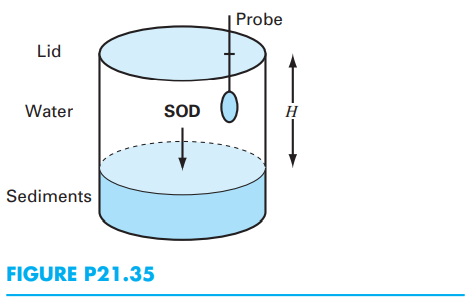
\includegraphics[width=0.50\textwidth]{pic.21.35}
	\label{pic.21.35}
\end{figure}
\begin{multicols}{2}

Based on the following data and $H$ = 0.1 m, use numerical differentiation to generate plots of \textbf{(a)} SOD versus
time and \textbf{(b)} SOD versus oxygen concentration:\\
\begin{tabular}{lccccccc}
	\hline

	\scriptsize{\textbf{$t$, d}} & \scriptsize{0} & \scriptsize{0.125} & \scriptsize{0.25} & \scriptsize{0.375} & \scriptsize{0.5} & \scriptsize{0.625} & \scriptsize{0.75}\\
	
	\scriptsize{\textbf{$o$, mg/L}} & \scriptsize{10} & \scriptsize{7.11} & \scriptsize{4.59} & \scriptsize{2.57} & \scriptsize{1.15} & \scriptsize{0.33} & \scriptsize{0.03}\\
	
	\hline
\end{tabular}

\textbf{21.36} The following relationships can be used to analyze
uniform beams subject to distributed loads:

{$$ \dfrac{dy}{dx} = \theta(x) \; \; \dfrac{d\theta}{dx} = \dfrac{M(x)}{EI} \; \; \dfrac{dM}{dx} = V(x) \; \; \dfrac{dV}{dx} = -\omega (x) $$}\\
where $x$ = distance along beam (m), $y$ = deflection (m),$\theta(x)$ = slope (m/m), E = modulus of elasticity (Pa = $N/m^2$),
I = moment of inertia ($m^4$), M(x) = moment (N m), V($x$) =
shear (N), and $w(x)$ = distributed load (N/m). For the case of
a linearly increasing load (recall Fig. P5.13), the slope can
be computed analytically as 
\begin{equation}
\tag{P21.36}
{\theta(x) = \dfrac{\omega_{0}}{120EIL}(-5x^4 + 6L^2x^2 - L^4)}
\end{equation}\\
Employ \textbf{(a)} numerical integration to compute the deflection
(in m) and \textbf{(b)} numerical differentiation to compute the
moment (in N m) and shear (in N). Base your numerical
calculations on values of the slope computed with
Eq. P21.36 at equally spaced intervals of $\Delta x = 0.125$ m along a 3-m beam. Use the following parameter values in
your computation: $E = 200$ GPa, $I = 0.0003 m^4$, and $\omega_{0} 2.5$ kN/cm. In addition, the deflections at the ends of the
beam are set at $y$(0) = $y$(L) = 0. Be careful of units.

\textbf{21.37} You measure the following deflections along the
length of a simply supported uniform beam (see Prob. 21.36)\\
\begin{tabular}{lcccc}
	\hline

	\textbf{$x$, m} \; 0 &  0.375 & 0.75 & 1.125 & 1.5\\

	\textbf{$y$, cm} \; 0 & -0.2571 & -0.9484 & -1.9689 & -3.2262\\
	
	\vspace{0,1in}\\
	
	\textbf{$x$, m} & 1.875 & 2.25 & 2.625 & 3\\
	
	\textbf{$y$, cm} & -4.6414 & -6.1503 & -7.7051 & -9.275\\

	\hline
\end{tabular}\\
Employ numerical differentiation to compute the slope, the
moment (in N m), the shear (in N) and the distributed load
(in N/m). Use the following parameter values in your computation: $E$ = 200 GPa, and $I$ = 0.0003 $m^4$.

\textbf{21.38} Evaluate $ \partial f/ \partial x $, $ \partial f / \partial y $, and $ \partial f (\partial x \partial ) $ for the following function at $x=y=1$ \textbf{(a)} analytically and \textbf{(b)} numerically $ \Delta x = \Delta y = 0.0001 $:

$ f(x,y) =3xy + 3x - x^3 - 3y^3 $

\textbf{21.39} Develop a script to generate the same computations
and plots as in Sec. 21.8, but for the following functions (for $ x= -3$ to 3 and $y = -3$ to 3): \textbf{(a)} $f(x,y) = e^{-(x^2+y^2)}$ and \textbf{(b)} $f(x,y) = xe^{ -(x^2+y^2) }$.

\textbf{21.40} Develop a script to generate the same computations
and plots as in Sec. 21.8, but for the MATLAB \texttt{peaks}
function over ranges of both $x$ and $y$ from –3 to 3.









\end{multicols}






	
	
	
	


\end{document}